\section{Model tornada Rankine}

Używany przez symulację model tornada został stworzony przez Williama Johna Macquorna Rankine  w połowie XIX wieku ~\cite{dbg_vortex}. Zakłada on, iż zaczynając od środka, czyli tzw. oka tornada, prędkość wiatru zwiększa się liniowo aż do osiągnięcia swojego maksimum przy promieniu R, a następnie wraz ze zwiększaniem promienia maleje wykładniczo. 

\begin{figure}[!h]
	\center
	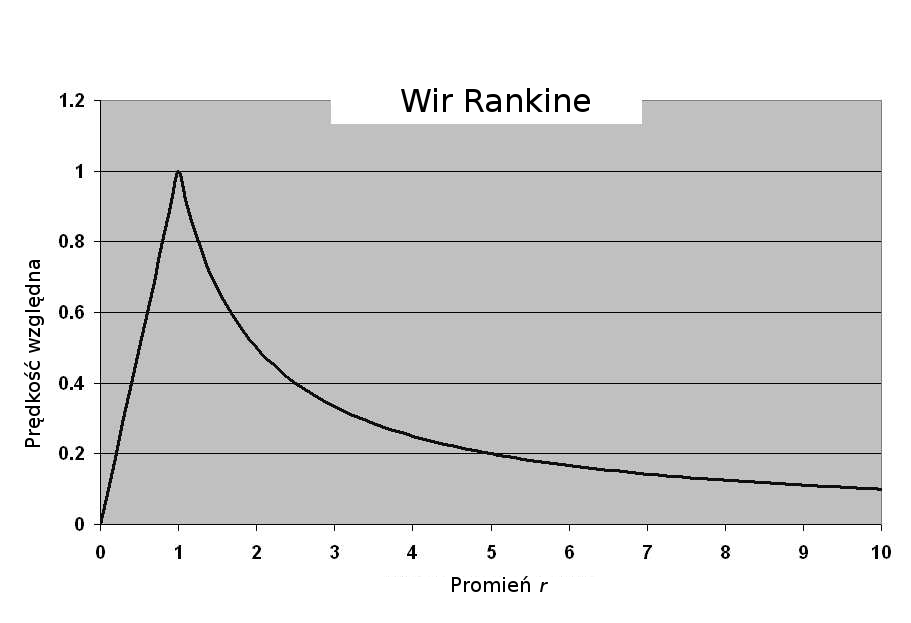
\includegraphics[scale=0.45]{rankine1}
	\caption{Zależność między prędkością wiatru a odległością od oka tornada. Źródło:~\cite{ktk_vortex}.}
	\label{fig:rankine1}
\end{figure} 

Zależności z wykresu przedstawionego na rysunku~\ref{fig:rankine1} reprezentowane są za pomocą równań współrzędnych biegunowych. Prędkość trawersalna (prędkość przemieszczania się w kierunku prostopadłym do promienia) opisana jest wzorem:
\begin{equation}
V_{\varphi}(r) =  \left\{ \begin{array}{ll}
\frac{V_{\varphi  max}\cdot r}{R_{max}} & \textrm{gdy $r \leq R_{max}$}\\
\frac{V_{\varphi  max}\cdot R_{max}}{r} & \textrm{gdy $r > R_{max}$}\\
\end{array} \right.
\end{equation}

gdzie

\begin{description}
  \item[$V_{\varphi}$] --  prędkość trawersalna (prędkość przemieszczania się w kierunku prostopadłym do promienia $r$)
  \item[${V_{\varphi  max}}$ ]-- maksymalna trawersalna prędkość wiatru
  \item[$r$ ]-- odległość punktu od środka tornada
  \item[$R_{max}$]-- maksymalny promień tornada
\end{description}

Podobnie do prędkości trawersalnej została opisana prędkość radialna. Różnicą jest to, iż iloraz promieni jest podniesiony do potęgi o wykładniku $0.6$. Stała ta została wyznaczona doświadczalnie za pomocą przenośnego radaru Dopplera~\cite{hb_doppler}.

\begin{equation}
V_{r}(r) =  \left\{ \begin{array}{ll}
V_{r  max}(\frac{r}{R_{max}})^{0.6} & \textrm{gdy $r \leq R_{max}$}\\
V_{r  max}(\frac{R_{max}}{r})^{0.6} & \textrm{gdy $r > R_{max}$}\\
\end{array} \right.
\end{equation}

gdzie

\begin{description}
  \item[$V_{r}$] --  prędkość radialna (prędkość zmiany długości promienia $r$)
  \item[${V_{r  max}}$ ]-- maksymalna radialna prędkość wiatru
  \item[$r$ ]-- odległość punktu od środka tornada
  \item[$R_{max}$]-- maksymalny promień tornada
\end{description}

Te dwie wielkości opisują model statycznego tornada. Aby przeprowadzić symulację tornada przechodzącego przez las, wprowadzony jest dodatkowy wektor prędkości -- prędkość translacji $V_{trans}$. Prędkość wiatru w modelu będzie wypadkową wszystkich tych trzech wielkości, przy czym wypadkowa prędkości trawersalnej $V_{\varphi}$ oraz prędkości radialnej $V_r$ nazywana jest prędkością cyrkularną $V_{cir}$.

\begin{figure}[!h]
	\center
	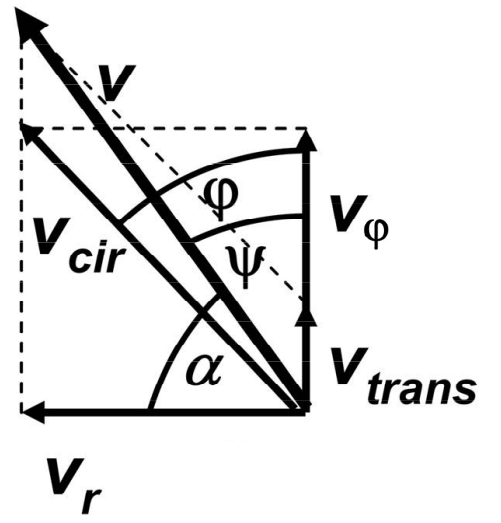
\includegraphics[scale=0.45]{rankine2}
	\caption{Składowe prędkości modelu tornada oraz ich wypadkowe. Źródło:~\cite{dpfh_model}.}
	\label{fig:rankine2}
\end{figure} 
